\begin{tikzpicture}
	\node() at (0,0) {
		\begin{tikzpicture}[scale=1,solid,black,
			declare function={
				hp(\x)= 2-2*sin(20*\x);	
				dev(\x) =  2-2*sin(20*\x) - max(2-2*sin(20*\x)-and(\x>1,\x<3)*1,0);
				zero(\x) = 0;		
			}]
			
			
			\begin{axis}[xmin=0,xmax=4.5,ymax=3, ymin=0, samples=500,width=4.5cm,height=3cm,
				axis x line*=bottom, axis y line*=left, axis lines=middle, xtick={1,2,3},xticklabels={$[$,$J$,$]$},ytick={1},yticklabels={$\varepsilon$}]
				\addplot[blue, ultra thick,domain=0:5] {hp(x)} node[above,pos=.5]{$h_p$};
				
				\addplot[domain=1:3.0001,red,dashed,thick,name path=F] {dev(x)};
				\addplot[name path=G] {zero(\x)};
				
				\addplot[pattern=north east lines, pattern color=red, thick]fill between[of=F and G];
			\end{axis}
			
		\end{tikzpicture}
	};

	\node() at (0,-2.2) {
		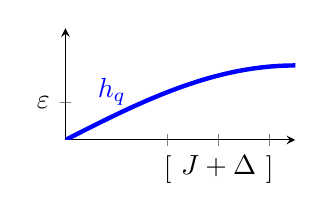
\begin{tikzpicture}[scale=1,solid,black,
			declare function={
				hq(\x)= 2*sin(20*\x);			
			}]
			
			
			\begin{axis}[xmin=0,xmax=4.5,ymax=3, ymin=0, samples=500,width=4.5cm,height=3cm,
				axis x line*=bottom, axis y line*=left, axis lines=middle, xtick={2,3,4},xticklabels={$[$,$J+\Delta$,$]$},ytick={1},yticklabels={$\varepsilon$}]
				\addplot[blue, ultra thick,domain=0:5] {hq(x)} node[above,pos=.2]{$h_q$};
			\end{axis}
			
		\end{tikzpicture}
	};

	\node() at (8,0) {
		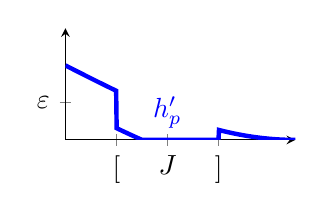
\begin{tikzpicture}[scale=1,solid,black,
			declare function={
				hp(\x)= max(2-2*sin(20*\x)-and(\x>1,\x<3)*1,0);			
			}]
			
			
			\begin{axis}[xmin=0,xmax=4.5,ymax=3, ymin=0, samples=500,width=4.5cm,height=3cm,
				axis x line*=bottom, axis y line*=left, axis lines=middle, xtick={1,2,3},xticklabels={$[$,$J$,$]$},ytick={1},yticklabels={$\varepsilon$}]
				\addplot[blue, ultra thick,domain=0:5] {hp(x)} node[above,pos=.5]{$h'_p$};
			\end{axis}
			
		\end{tikzpicture}
	};
	
	\node() at (8,-2.2) {
		\begin{tikzpicture}[scale=1,solid,black,
			declare function={
				hq(\x)= 2*sin(20*\x) + 2-2*sin(20*(\x-1)) - max(2-2*sin(20*(\x-1))-and(\x>2,\x<4)*1,0);	
				dev(\x)= 2*sin(20*\x);		
			}]
			
			
			\begin{axis}[xmin=0,xmax=4.5,ymax=3, ymin=0, samples=500,width=4.5cm,height=3cm,
				axis x line*=bottom, axis y line*=left, axis lines=middle, xtick={2,3,4},xticklabels={$[$,$J+\Delta$,$]$},ytick={1},yticklabels={$\varepsilon$}]
				\addplot[blue, ultra thick,domain=0:5,name path=G] {hq(x)} node[above,pos=.2]{$h'_q$};
				
				\addplot[domain=2:4,red,dashed,thick,name path=F] {dev(x)};
				
				\addplot[domain=2:4,pattern=north east lines, pattern color=red, thick]fill between[of=F and G];
			\end{axis}
			
		\end{tikzpicture}
	};

	\draw[->,ultra thick] (2.5,-1.2) -- node[above]{$\varepsilon$-deviation} node[below]{$(q,J,\varepsilon,\Delta) \in A_p(h)$} (5.5,-1.25);
\end{tikzpicture}